% Autor: Francisco Javier Barranco Tena
% State of the Art
% Alt + z o Option + z para activar el word wrap en Visual Studio Code

Detectar el estado del pavimento presenta desafíos significativos que han sido abordados mediante diversas soluciones. Entre estas soluciones se incluyen la integración de sensores de acelerómetros en vehículos\cite{Pavement_Anomalies_Accelerometer}, la aplicación de sistemas basados en LIDAR\cite{LIDAR_Blasiis}\cite{LIDAR_VanDerHorst}, y el desarrollo de sistemas fundamentados en \textit{Computer Vision}. Los avances recientes en algoritmos de detección de objetos, como YOLO (\textit{You Only Look Once}), han mejorado notablemente la eficacia de los sistemas basados en \textit{Computer Vision}. Además, estos sistemas no requieren una inversión significativa en hardware específico, ya que pueden emplearse con cámaras convencionales, como las de teléfonos móviles o las cámaras de vehículos.

\section{Soluciones basadas en \textit{Computer Vision}}
En el ámbito de soluciones fundamentadas en \textit{Computer Vision}, destaca la CRDDC (Crowdsensing-based Road Damage Detection Challenge), una competición que ha tenido lugar en los años 2018, 2020 y 2022. El propósito de la CRDDC radica en la implementación de sistemas de \textit{Computer Vision} capaces de utilizar cámaras de teléfonos móviles y vehículos para inspeccionar el estado del pavimento en cualquier parte del mundo. Esta competición proporciona un extenso conjunto de datos compuesto por decenas de miles de imágenes anotadas, así como un método de evaluación que facilita la comparación de los modelos desarrollados con aquellos implementados durante la competición. Los datos y las métricas de evaluación de la CRDDC 2022 componen el marco de evaluación que se usara durante la implementación del sistema base de este TFG. En las secciones \ref{SEC:DATOS} y \ref{SEC:METRICAS} se entra en detalle sobre este marco de evaluación.

En el artículo “Crowdsensing-based Road Damage Detection Challenge (CRDDC’2022)” \cite{CRDDC2022_paper}, se explica de forma resumida las soluciones propuestas por los once equipos líderes de la competición CRDDC 2022. Dentro de esta lista de soluciones propuesta, destaca que casi todas las soluciones utilizan \textit{ensembles}\footnote{Técnica que combina múltiples modelos de aprendizaje automático para mejorar la precisión y robustez del sistema. Estos conjuntos pueden incluir diferentes tipos de modelos o utilizar diferentes conjuntos de datos, lo que permite obtener predicciones más confiables y generalizables. En español, se puede entender como 'conjunto' o 'ensamblaje' de modelos.} basados principalmente en modelos YOLO (\textit{You Only Look Once}). 

En la figura \ref{fig:CRDDC2022_detailed_solutions} se muestra una tabla con los detalles de las soluciones propuestas por los equipos líderes de la CRDDC 2022. Se observa que todos los equipos han incorporado alguna versión de YOLO en sus soluciones y casi todos han utilizado \textit{ensembles} para mejorar la precisión de sus modelos. Otra característica destacada es la modificación en la arquitectura de YOLO, como la utilización de \textit{custom anchor boxes}, el uso de \textit{Atrous Spatial Pyramid Pooling} y la implementación de distintos mecanismos de atención. Además, se han empleado técnicas de \textit{data augmentation}, el uso de pesos pre-entrenados y técnicas de \textit{transfer learning}. Estas estrategias han permitido a los equipos mejorar significativamente la precisión y robustez de sus modelos para la detección de daños en pavimentos.

% Añadir la tabla de soluciones de la CRDDC 2022
\begin{figure}[H]
    \centering
    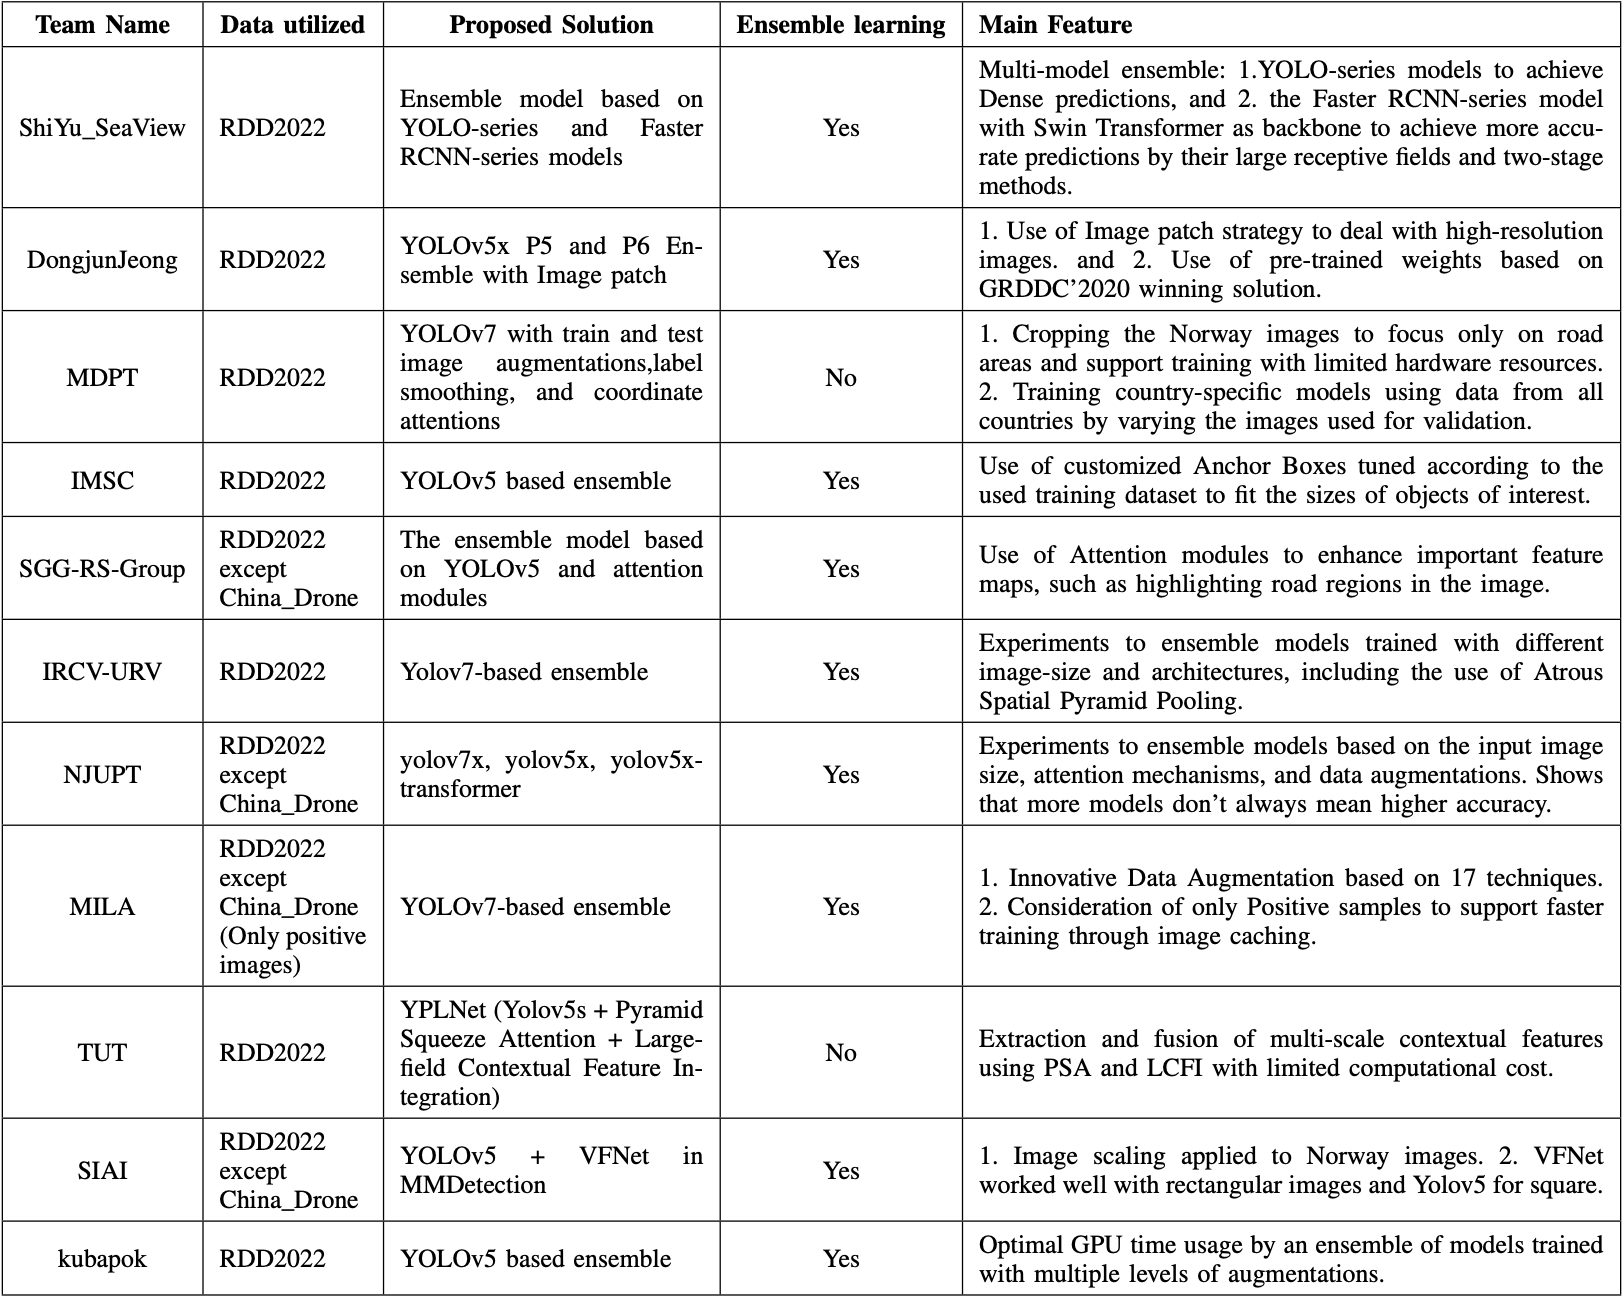
\includegraphics[width=1\textwidth]{../img/winner-solutions.png}
    \caption{Detalles de las soluciones propuestas por los top 11 equipos de la CRDDC 2022. Table IV de 'Crowdsensing-based Road Damage Detection Challenge (CRDDC’2022)' \cite{CRDDC2022_paper}.}
    \label{fig:CRDDC2022_detailed_solutions}
\end{figure}

Adicionalmente, el artículo "From global challenges to local solutions: A review of cross-country collaborations and winning strategies in road damage detection." \cite{CRDDC2022_review} proporciona un resumen de las soluciones y aprendizajes de la edición de 2022 de la competición. Durante este TFG utilizaremos los datos, soluciones propuestas, aprendizajes y métricas de la CRDDC 2022 para desarrollar un modelo de detección del estado del pavimento.

Generalmente, en competiciones como la CRDDC, los modelos ganadores suelen ser \textit{ensembles} complejos que combinan múltiples modelos de detección de objetos. Estos \textit{ensembles} suelen combinar modelos de diferentes arquitecturas, como YOLO, Faster R-CNN, o EfficientDet, y se entrenan utilizando técnicas de \textit{transfer learning}. En este trabajo buscaremos implementar un modelo más simple que no requiera tantas capacidades computacionales, pero que sea capaz de detectar daños en el pavimento con una buena precisión y eficacia en tiempo real. El objetivo es entrenar un modelo base que sirva como punto de partida para futuras soluciones de detección del estado del pavimento.


\section{Modelo de detección de objetos: YOLOv8}
Como se ha mencionado, en la CRDDC 2022 destaco el uso de los modelos YOLO. YOLO \cite{YOLO} es un modelo de detección de objetos en tiempo real que divide la imagen en una cuadrícula y predice las cajas delimitadoras y las clases de los objetos en cada celda de la cuadrícula. En este TFG se utilizará la implementación de YOLOv8 de Ultralytics \cite{yolov8_ultralytics}, que es una de las implementaciones más avanzadas y eficientes de YOLO. La librería de Python de Ultralytics proporciona una interfaz sencilla para entrenar, validar e inferir con modelos YOLO.

YOLOv8 es el modelo más reciente y avanzado de la familia YOLO (\textit{You Only Look Once}), diseñado para tareas de detección de objetos, clasificación de imágenes y segmentación de instancias. Desarrollado por Ultralytics, la misma organización que creó el influyente y definitorio modelo YOLOv5, YOLOv8 incorpora numerosas mejoras arquitectónicas y de experiencia para los desarrolladores en comparación con su predecesor. La serie de modelos YOLO ha sido famosa en el mundo de la visión por computadora debido a su considerable precisión manteniendo un tamaño de modelo pequeño, permitiendo su entrenamiento en una sola GPU y su despliegue a bajo costo.

YOLOv8 destaca por su alta precisión, medida por los \textit{benchmarks} de Microsoft COCO \cite{COCO} y Roboflow 100 \cite{Roboflow100}. Microsoft COCO es un conjunto de datos de referencia ampliamente utilizado para evaluar modelos de visión por computadora, mientras que Roboflow 100 evalúa el rendimiento del modelo en diversos dominios específicos de tareas. Por ejemplo, el modelo \textit{medium} de YOLOv8 (YOLOv8m) alcanza un 50.2\% mAP en COCO y tiene un rendimiento sustancialmente mejor que YOLOv5 en Roboflow 100. Además, YOLOv8 ofrece numerosas características convenientes para desarrolladores, incluyendo una CLI\footnote{Command Line Interface o Interfaz de Línea de Comandos es un mecanismo de software que permite interactuar con un programa mediante comandos escritos en texto plano desde una terminal.} fácil de usar y un paquete Python bien estructurado, facilitando el entrenamiento y la implementación de modelos. La comunidad de usuarios de YOLO es extensa y en crecimiento, brindando soporte y orientación. Estas ventajas hacen de YOLOv8 una opción robusta y accesible para proyectos de visión por computadora.

\subsection{Arquitectura de YOLOv8}
La arquitectura de YOLOv8 aún no cuenta con un artículo publicado, por lo que no disponemos de información directa sobre la metodología de investigación y los estudios de \textit{ablation}\footnote{Ablation o ablación en el contexto de \textit{deep learning} se refiere a la técnica de eliminar o modificar partes del modelo para evaluar su impacto en el rendimiento, ayudando a identificar la importancia de diferentes componentes y optimizar el diseño del modelo.} realizados durante su creación. No obstante, la comunidad ha analizado el repositorio y la información disponible para documentar las novedades de YOLOv8. En la figura \ref{fig:YOLOv8_architecture} se puede ver una visualización de la arquitectura de YOLOv8 creada por el usuario de GitHub RangeKing\cite{RangeKing_GitHub}. A continuación, comentaré los detalles más importantes de la arquitectura de YOLOv8 y sus novedades respecto a versiones anteriores. \cite{whats-new-in-yolov8} \cite{yolov8-architecture-blog} \cite{yolov8-architecture-blog2}

La arquitectura de YOLOv8 se divide en dos componentes principales: el \textit{backbone} y el \textit{head}. El \textit{backbone} extrae características de las imágenes de entrada mediante convoluciones y otras operaciones. El \textit{head} fusiona estas características y realiza las predicciones finales de detección de objetos, clasificación y segmentación. A veces, el \textit{head} se subdivide en dos partes: el \textit{neck}, que fusiona las características extraídas por el \textit{backbone}, y el \textit{head}, que realiza las predicciones. En la figura \ref{fig:YOLOv8_architecture}, el \textit{neck} corresponde a todo lo marcado como \textit{head}, excepto los bloques de Detect, que constituyen el verdadero \textit{head}. La figura \ref{fig:YOLOv8_architecture_neck_head} muestra una visualización alternativa de la arquitectura de YOLOv8 con el \textit{neck} y el \textit{head} separados.

% Añadimos la figura con la arquitectura de YOLOv8 creada por RangeKing
\begin{figure}
    \centering
    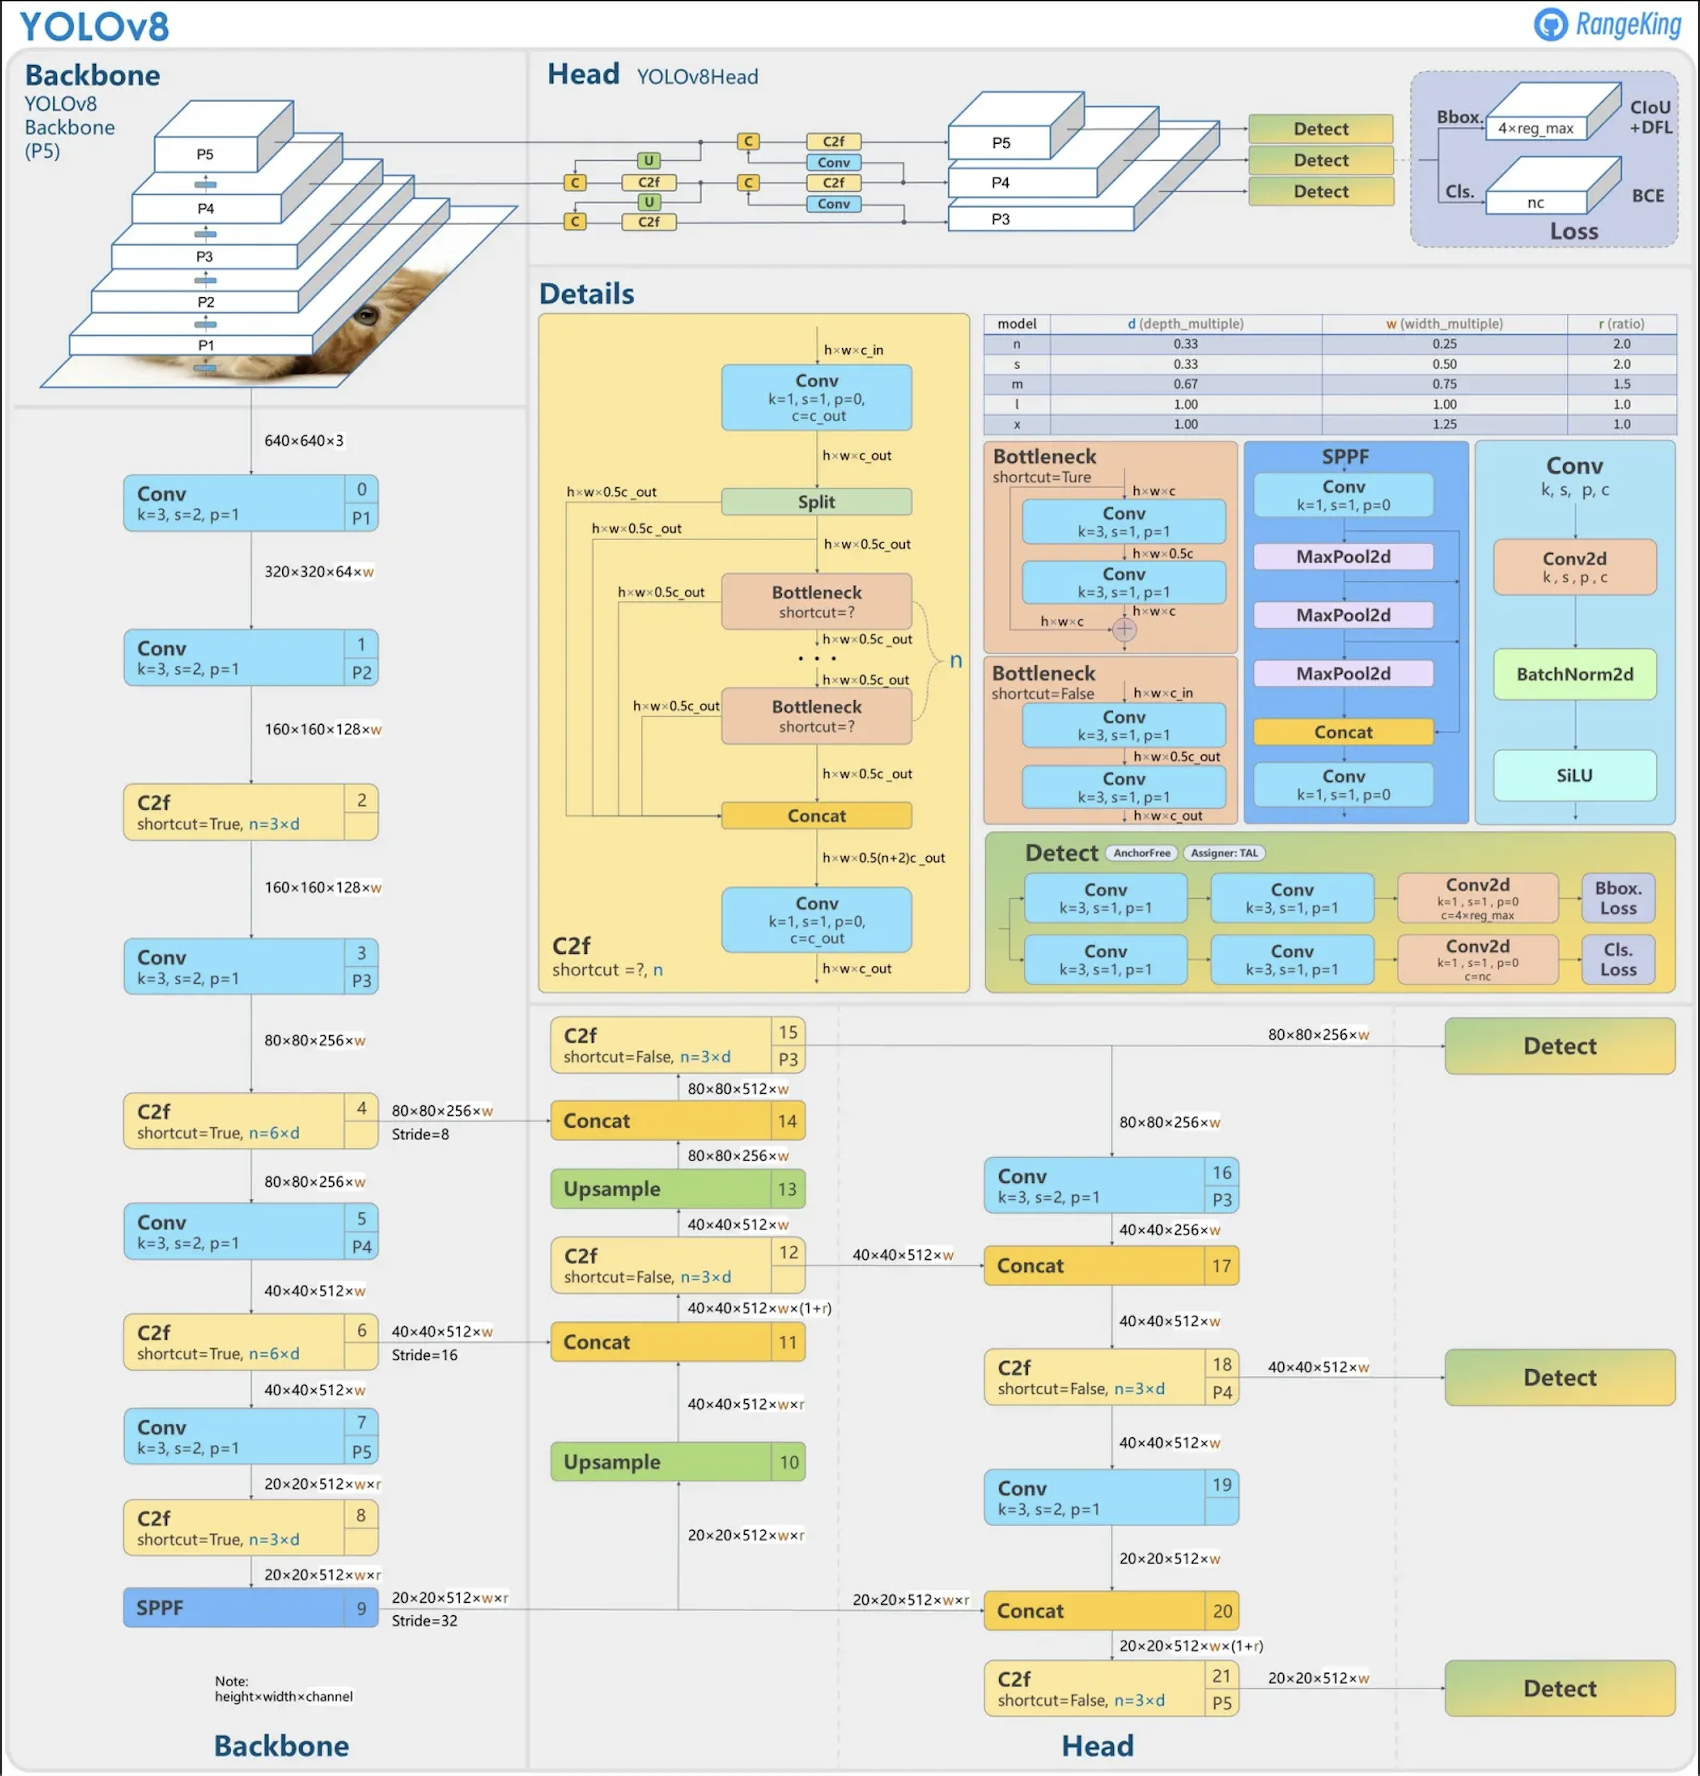
\includegraphics[width=1\textwidth]{../img/yolov8-arq.png}
    \caption{Arquitectura de YOLOv8, visualización realizada por el usuario de GitHub RangeKing\cite{RangeKing_GitHub}.}
    \label{fig:YOLOv8_architecture}
\end{figure}

El \textit{backbone} en una red neuronal convolucional (CNN) es responsable de extraer características de las imágenes de entrada. Consiste en una serie de capas de convolución y otras operaciones que transforman la imagen original en un mapa de características de alta dimensión, capturando información relevante sobre la estructura y contenido de la imagen.

En YOLOv8, el \textit{backbone} se basa en la arquitectura CSPDarknet53. Este \textit{backbone} utiliza conexiones parciales entre etapas (\textit{Cross Stage Partial connections}) que mejoran el flujo de información entre capas, incrementando la capacidad de aprendizaje y eficiencia del modelo. En la figura \ref{fig:YOLOv8_architecture}, el \textit{backbone} se representa con bloques de diferentes colores que indican las distintas capas y módulos utilizados: capas de convolución estándar (Conv) con varias configuraciones de kernel y \textit{stride}, bloques con atajos internos (C2f) que mejoran la transferencia de información y facilitan el aprendizaje de características complejas, y un bloque de \textit{Spatial Pyramid Pooling Fusion} (SPPF) que captura información contextual de diferentes escalas espaciales. El \textit{backbone} de YOLOv8 se compone de varios bloques denominados P1, P2, P3, P4 y P5, cada uno de los cuales representa un nivel de procesamiento de características. En las primeras etapas, P1 y P2 (a veces llamado \textit{stem}), se aplican convoluciones con diferentes tamaños de kernel y \textit{strides} para reducir la resolución de las imágenes y extraer características básicas. A medida que avanzamos a P3 y P4, el modelo emplea bloques C2f que permiten conexiones de atajo internas, mejorando la transferencia de información y facilitando el aprendizaje de características más complejas.  Estas etapas también incluyen operaciones de concatenación que combinan características de diferentes capas. Finalmente, en P5, se utiliza una combinación de convoluciones, capas de concatenación y un bloque SPPF que ayuda a capturar información contextual de diferentes escalas espaciales.

El \textit{neck} en una arquitectura CNN se encarga de fusionar los mapas de características provenientes de diferentes etapas del \textit{backbone}. En el caso de YOLOv8, el \textit{neck} utiliza característica de P3, P4 y P5. Su objetivo es combinar información de múltiples escalas para mejorar la capacidad del modelo para detectar objetos de diferentes tamaños. Al reunir características semánticas de alto nivel con información espacial de bajo nivel, el \textit{neck} permite al modelo manejar mejor la diversidad en tamaño y forma de los objetos presentes en las imágenes.

En YOLOv8, el \textit{neck} utiliza el mismo módulo C2f empleado en el \textit{backbone} para facilitar la fusión de características de diferentes niveles de abstracción, mejorando la precisión de detección, especialmente para objetos pequeños. En los diagramas proporcionados, el \textit{neck} se representa como las capas que realizan operaciones de concatenación (Concat) y \textit{upsampling} (Upsample). Las operaciones de concatenación combinan características de múltiples capas para capturar información a varias escalas, mientras que las operaciones de \textit{upsampling} aumentan la resolución de los mapas de características para fusionarlos adecuadamente.

El \textit{head} en una arquitectura CNN es la parte encargada de realizar las predicciones finales. Genera las coordenadas de las cajas delimitadoras (\textit{bounding boxes}), las puntuaciones de objetividad (\textit{objectness scores}) y las probabilidades de clase para cada objeto detectado. Esta etapa es crucial, ya que convierte las características procesadas y fusionadas en etapas anteriores en información útil para la detección de objetos. Una de las principales novedades de YOLOv8 es que su \textit{head} es \textit{anchor-free}, lo que significa que no utiliza \textit{anchor boxes} predefinidas para realizar las predicciones. En lugar de eso, el modelo predice directamente el centro de los objetos y las dimensiones de las cajas delimitadoras. A continuación, se profundiza en esta característica y sus implicaciones.


\subsection{Detección de objetos sin \textit{anchor boxes} en YOLOv8}
La predicción basada en \textit{anchor boxes} utiliza cajas delimitadoras predefinidas como puntos de partida para ajustar y localizar objetos en una imagen. En este enfoque, se generan múltiples \textit{anchor boxes} alrededor de la imagen y el modelo predice desajustes desde estas cajas para identificar objetos. En contraste, la predicción libre de \textit{anchor boxes}, como la utilizada en YOLOv8, omite estos puntos de partida predefinidos y predice directamente el centro de los objetos, luego se predice el largo, ancho y rotación de la caja centrada en el objeto. Este método simplifica el proceso de predicción, reduce la complejidad computacional y mejora la precisión, especialmente en casos con objetos de formas y tamaños irregulares. Ver la figura \ref{fig:anchor-box-free} para una comparación visual de la predicción con y sin \textit{anchor boxes}.

La predicción sin \textit{anchor boxes} elimina la necesidad de configurar y ajustar manualmente los \textit{anchor boxes}, reduciendo la complejidad computacional y mejorando la velocidad de convergencia durante el entrenamiento. Además, esta metodología puede mejorar la generalización del modelo a nuevos conjuntos de datos, ya que no depende de una distribución específica de \textit{anchor boxes}. En resumen, YOLOv8 ofrece una solución más versátil y poderosa para la detección de objetos, adaptándose mejor a una variedad más amplia de escenarios.

% Añadimos la figura de anchorfree-vs-anchorbox
\begin{figure}[H]
    \centering
    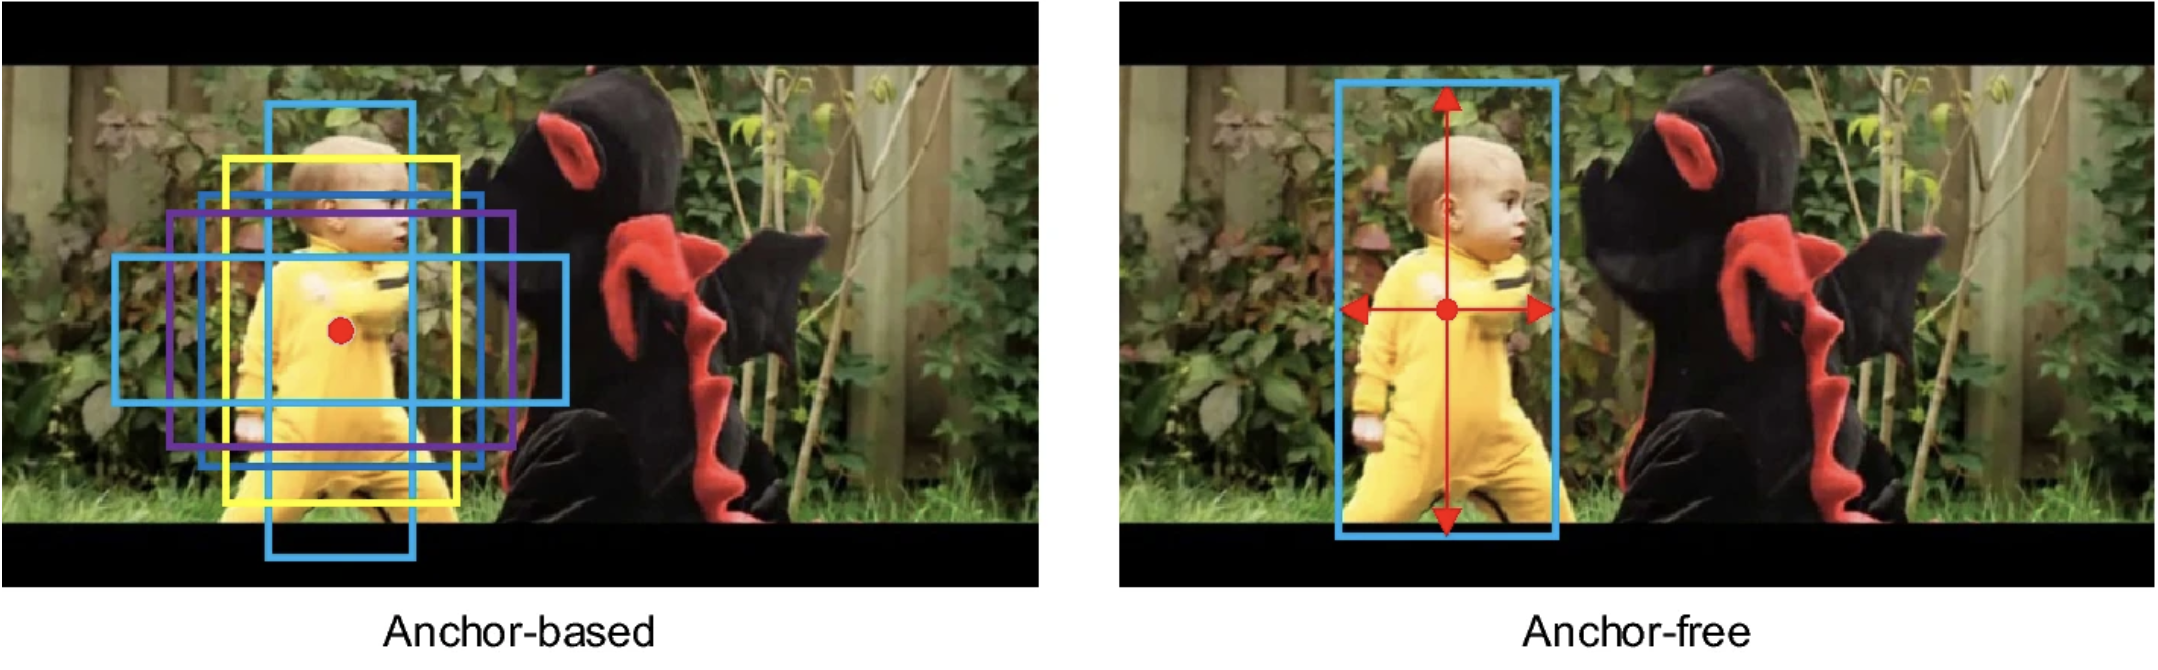
\includegraphics[width=1\textwidth]{../img/anchorfree-vs-anchorbox.png}
    \caption{Predicción de objetos con y sin \textit{anchor boxes}. Figura extraída de \cite{SiameseAnchorFree}.}
    \label{fig:anchor-box-free}
\end{figure}
